\chapter{Diseño del algoritmo}\label{ch:diseno-algoritmo}


\section{Lenguaje}\label{sec:lenguaje}

En este apartado iremos pasando por todos los lenguajes que se han diseñado y
probado hasta llegar al lenguaje escogido para la representación del problema. Un
lenguaje candidato tiene que poder realizar todos los movimientos posibles del
cubo de Rubik y a la vez tiene que realizar las comprobaciones suficientes para
determinar qué movimiento realizar en cada momento. Es por ello que el lenguaje
constará de sentencias condicionales, capaces de ejecutar una rama si la
condición se cumple y sentencias de acción como puede ser el desplazamiento de
una cierta cara en un cierto sentido.

\subsection{Solución 1: El cubo como mapa}\label{subsec:solucion1}

El primer lenguaje que se nos planteó, fue al imaginar un lenguaje parecido al
lenguaje del problema de la hormiga. El problema de la hormiga tiene los
operadores de movimiento de la hormiga por el mapa y las comprobaciones de
existencia de comida enfrente. Adaptando este problema a nuestro problema,
podríamos pensar en el cubo de Rubik como un mapa bidimensional. Un mapa con
forma de cruz, donde cada casilla del cubo representa una posición del mapa.
Sobre este mapa nos podemos mover hacia arriba, hacia abajo, derecha e izquierda.
Al situarnos en el borde de una cara y avanzar nos situaremos en la siguiente
cara, es decir, no existe límite, siempre podemos avanzar.

Una vez que nos podemos desplazar por el mapa, como la hormiga, querremos
realizar ciertas comprobaciones en relación a nuestra posición actual, como por
ejemplo si existe comida en nuestra posición. En el caso del cubo de rubik,
querremos  comprobar el color de la pegatina en la que estemos situados.

Una vez que tenemos la funcionalidad de comprobar cualquier casilla de nuestro
cubo de Rubik, los siguientes operadores son triviales y básicos para el
resolvedor del cubo de Rubik: los movimientos de cara. Estos son los operadores
que rotan una cara, por ejemplo, el que rota la cara derecha en sentido de las
agujas del reloj.

Es normal pensar qué parámetros son necesarios en nuestro sistema, es decir,
cuando movemos una cara necesitaremos especificar qué cara movemos. Debe existir
el operador “mover” y el parámetro “cara” que especifica que cara movemos. No
obstante, el objetivo de este lenguaje es conseguir un lenguaje gramaticalmente
libre, de tal forma que cualquier nodo sea compatible con otro.

Este hecho tiene la ventaja de que cualquier nodo puede sustituir a otro, por
eso, los operadores de mutación y cruzamiento requieren de menos esfuerzo para
llevar a cabo con éxito su labor. Por lo tanto, en el lenguaje tendremos nodos
del tipo “IfBlue”, “IfRed” o MoveFaceUpClockwise.

De esta forma tenemos el conjunto de nodos terminales que se muestra en la
tabla \ref{tab:n-terminales-sol1} y en la figura \ref{fig:leng1nodosterm}, y el
conjunto de nodos no-terminales en la tabla \ref{tab:n-noterminales-sol1} y en
la figura \ref{fig:leng1nodosnoterm}.


\begin{table}[t]
\caption{Tabla de nodos terminales de la solución 1.}
\label{tab:n-terminales-sol1}
\centering
\begin{tabular}{lp{8cm}}
\toprule
\textbf{Nombre} & \textbf{Descripción}\\
\midrule
\textbf{MovePosUp}					&	Mueve la posición actual a la casilla superior. Si no
existe tal casilla, se saltará de cara a la superior a la casilla Y2. Si
estamos en la cara superior, nos desplazaremos a la cara trasera.\\ \hline
\textbf{MovePosDown}				&	Mueve la
posición actual a la casilla inferior. Si no existe tal casilla, se saltará de
cara a la inferior a la casilla Y0. Si estamos en la cara inferior, nos
desplazaremos a la cara trasera.\\\hline
\textbf{MovePosLeft}				&	Mueve la posición actual a la casilla izquierda. Si
no existe tal casilla, se saltará de cara a la izquierda a la casilla
X2.\\\hline \textbf{MovePosRight}				&	Mueve la posición actual a la casilla derecha. Si no
existe tal casilla, se saltará de cara a la derecha a la casilla X0. \\\hline
\textbf{MoveFaceUpClockwise}			&	Mueve la cara superior en el sentido de las
agujas del reloj.\\\hline
\textbf{MoveFaceDownClockwise}		&	Mueve la cara inferior en el sentido de las
agujas del reloj.\\\hline
\textbf{MoveFaceRightClockwise}		&	Mueve la cara derecha en el sentido
de las agujas del reloj.\\\hline
\textbf{MoveFaceLeftClockwise}		&	Mueve la cara izquierda en
el sentido de las agujas del reloj.\\\hline
\textbf{MoveFaceFrontClockwise}		&	Mueve la cara
frontal en el sentido de las agujas del reloj. \\\hline
\textbf{MoveFaceBackClockwise}		&	Mueve la cara trasera en el sentido de las
agujas del reloj.\\\hline
\textbf{MoveFaceUpCounterClockwise}&	Mueve la cara superior en el sentido
opuesto a las agujas del reloj.\\\hline
\textbf{MoveFaceDownCounterClockwise}&	Mueve la cara inferior en
el sentido opuesto a las agujas del reloj.\\\hline
\textbf{MoveFaceRightCounterClockwise}&	Mueve
la cara derecha en el sentido opuesto a las agujas del reloj.\\\hline
\textbf{MoveFaceLeftCounterClockwise}&	Mueve la cara izquierda en el sentido
opuesto a las agujas del reloj.\\\hline
 \textbf{MoveFaceFrontCounterClockwise}&	Mueve la cara frontal en
el sentido opuesto a las agujas del reloj.\\\hline
 \textbf{MoveFaceBackCounterClockwise}&Mueve
la cara trasera en el sentido opuesto a las agujas del reloj.\\
\bottomrule
\end{tabular}
\end{table}


\begin{table}[t]
\caption{Tabla de nodos no-terminales de la solución 1.}
\label{tab:n-noterminales-sol1}
\centering
\begin{tabular}{lcp{8cm}}
\toprule
\textbf{Nombre}&\textbf{Aridad}& \textbf{Descripción}\\
\midrule
\textbf{IfBlue}&2&	Comprueba que la casilla de la posición actual sea azul. Si
es así ejecuta lo hijos de la izquierda. Si no, ejecuta los de la
derecha.\\\hline
\textbf{IfWhite}&	2& Comprueba que la casilla de la posición actual sea blanca.
Si es así ejecuta lo hijos de la izquierda. Si no, ejecuta los de la
derecha.\\\hline
\textbf{IfGreen}&2& Comprueba que la casilla de la posición actual sea verde.
Si es así ejecuta lo hijos de la izquierda. Si no, ejecuta los de la derecha.
\\\hline
\textbf{IfOrange}&	2&	Comprueba
que la casilla de la posición actual sea naranja. Si es así ejecuta lo hijos de
la izquierda. Si no, ejecuta los de la derecha.\\ \hline
\textbf{IfRed}&	2&	Comprueba que la
casilla de la posición actual sea rojo. Si es así ejecuta lo hijos de la
izquierda.Si no, ejecuta los de la derecha.\\\hline
\textbf{IfYellow}&	2&	Comprueba que la
casilla de la posición actual sea amarillo. Si es así ejecuta lo hijos de la
izquierda. Si no, ejecuta los de la derecha. \\\hline
\textbf{Progn2}&	2&	Ejecuta primero la rama
izquierda y luego la derecha.\\\hline
\textbf{Progn3}&	3&	Ejecuta primero la rama izquierda,
luego la central y luego la derecha.\\
\bottomrule
\end{tabular}
\end{table}


\begin{figure}[t]
\centering
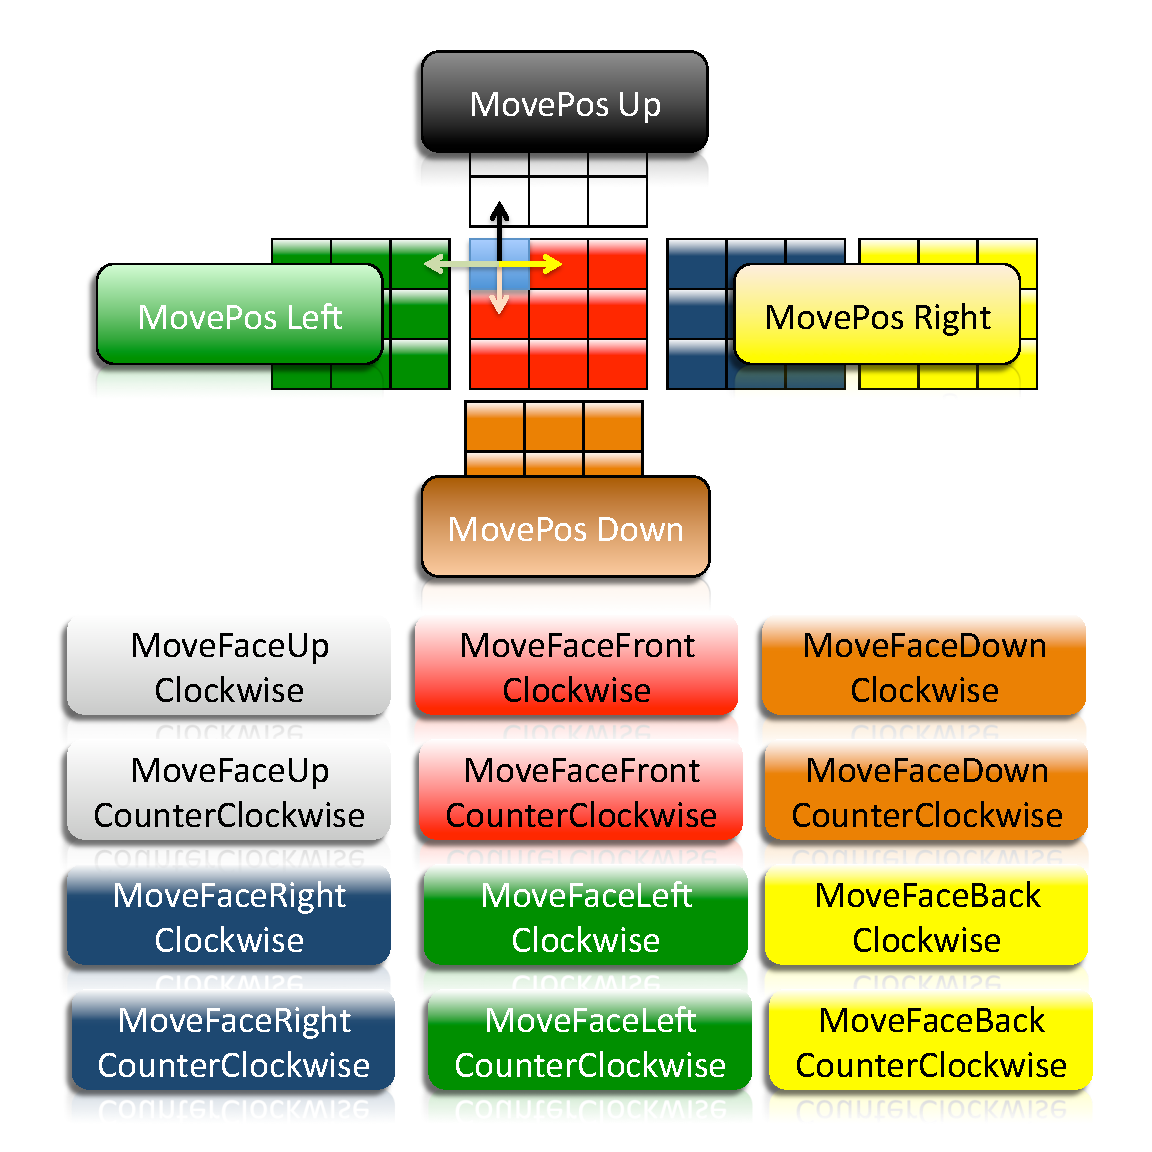
\includegraphics[width=0.65\textwidth]{figs/pdf/leng1nodosterm}
\caption{Nodos terminales de la solución 1.}
\label{fig:leng1nodosterm}
\end{figure}

\begin{figure}[t]
\centering
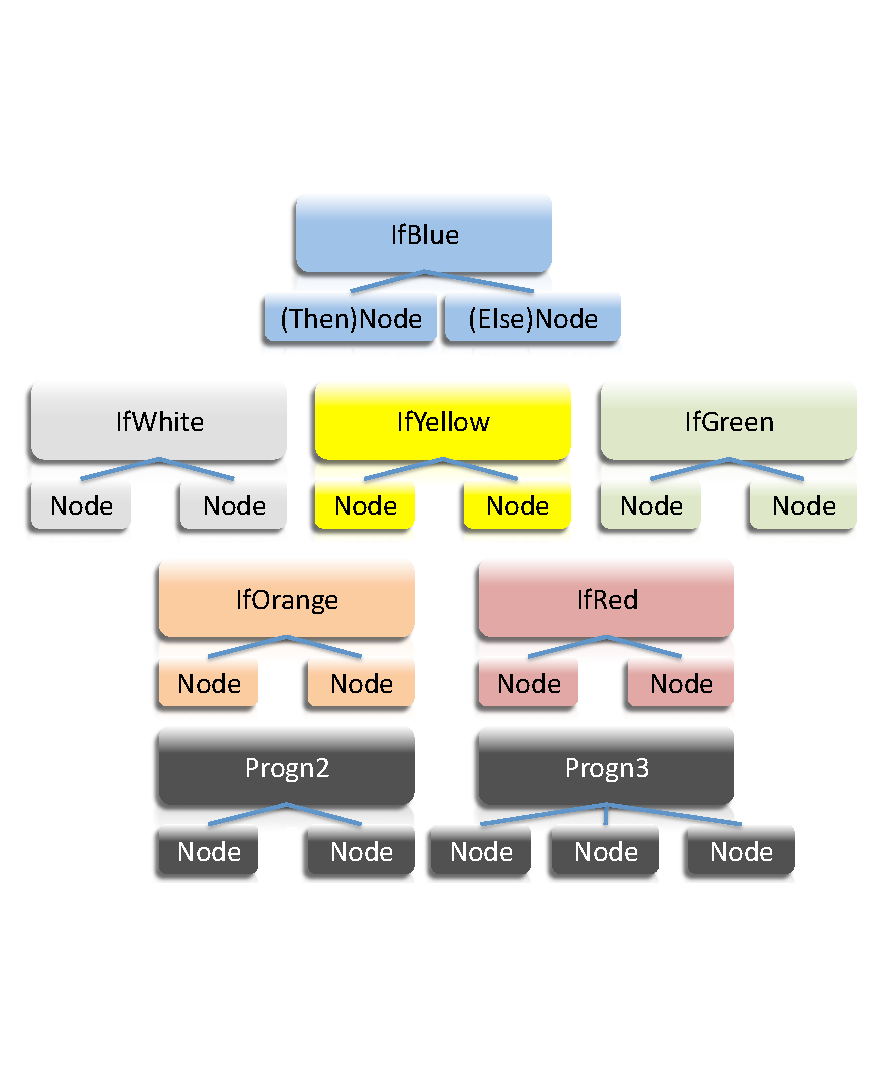
\includegraphics[width=0.65\textwidth]{figs/pdf/leng1nodosnoterm}
\caption{Nodos no terminales de la solución 1.}
\label{fig:leng1nodosnoterm}
\end{figure}



Este lenguaje ofrece la ventaja que cada nodo es sustituible por cualquier otro.
De esta manera, la generación de árboles, cruzamiento, mutación y cualquier
operador que trabaje con el lenguaje resultará beneficiado de esta situación.

Sin embargo este lenguaje resulta poco eficiente, en cuanto al número de nodos
requeridos para lograr resolver cubos, ya que el trabajo que cuesta comprobar dos
casillas diferentes no siempre es el mismo, de modo que alcanzar el camino hacia
una casilla puede convertirse en otro problema de cierta complejidad en si mismo.

Además, al ser necesario saber en que posición estamos, es inherente que el
estado del sistema entre en juego a la hora de determinar los resultados de un
operador. Es por esto que este lenguaje es difícilmente predecible y entendible
por el hombre.

Por otra parte, este es un lenguaje débilmente tipado de forma que la aparición
de bloat estará mucho más presente, y podrá ocupar un espacio mucho mayor en los
árboles del sistema.

Vamos a ver un ejemplo de cómo se podría solucionar un cubo de Rubik de nivel 1
(una cara desplazada respecto de la solución, figura \ref{fig:leng1ejemplo1})
con este lenguaje. Si, por ejemplo, rotamos la cara de la izquierda en el sentido de las agujas del reloj, tendremos
un cubo de Rubik de nivel 1, donde la cara frontal tiene tres casillas del color
de la cara superior, la cara inferior tiene 3 casillas del color de la cara
frontal y así sucesivamente. Para dar con la solución bastaría con el siguiente
plan:

\begin{algorithmic}
\IF {$Orange$} 
        \STATE $MovePosDown$
        \STATE $MovePosDown$
        \STATE $MovePosDown$
        \STATE $MovePosRight$
        \IF {$Orange$}
                \STATE $MoveFaceLeftCounterClockwise$
        \ENDIF
\ENDIF 
\end{algorithmic}

El plan puede no parecer muy complicado, pero si queremos volver a evaluar la
casilla inicial, tendremos que volver hacia atrás y repetirlo del mismo modo con
todas las casillas que se tengan que comprobar. Por otra parte, el lenguaje
admite sentencias del tipo 
\begin{algorithmic}
\IF {$IfOrange$} 
        \IF {$IfRed$}
                \STATE \ldots
        \ENDIF
\ENDIF 
\end{algorithmic} 
(figura \ref{fig:leng1ejemplo2}) que carecen de sentido y que son
difícilmente controlables. Esto puede desencadenar la generación de mucho código
sin sentido que carezca de utilidad.




\begin{figure}[t]
\centering
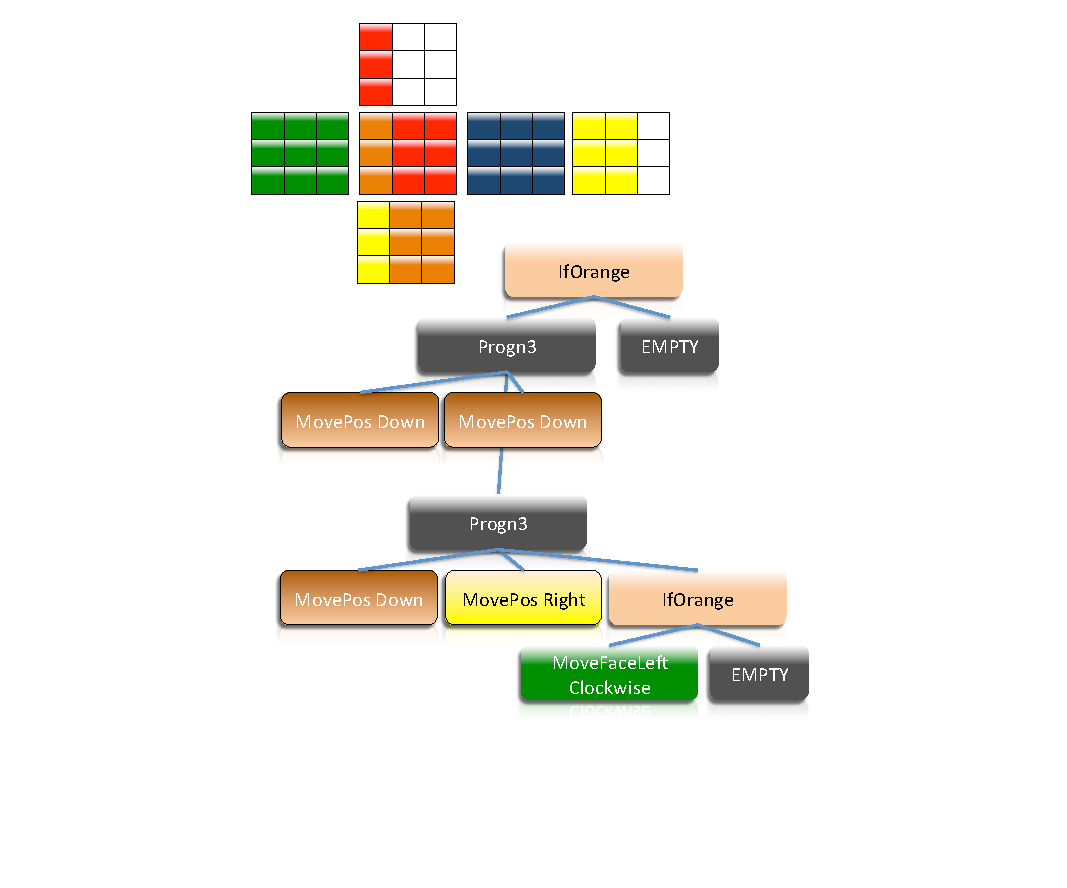
\includegraphics[width=0.65\textwidth]{figs/pdf/leng1ejem1}
\caption{Ejemplo de árbol que resuelve un cubo de rubik de nivel 1.}
\label{fig:leng1ejemplo1}
\end{figure}

\begin{figure}[t]
\centering
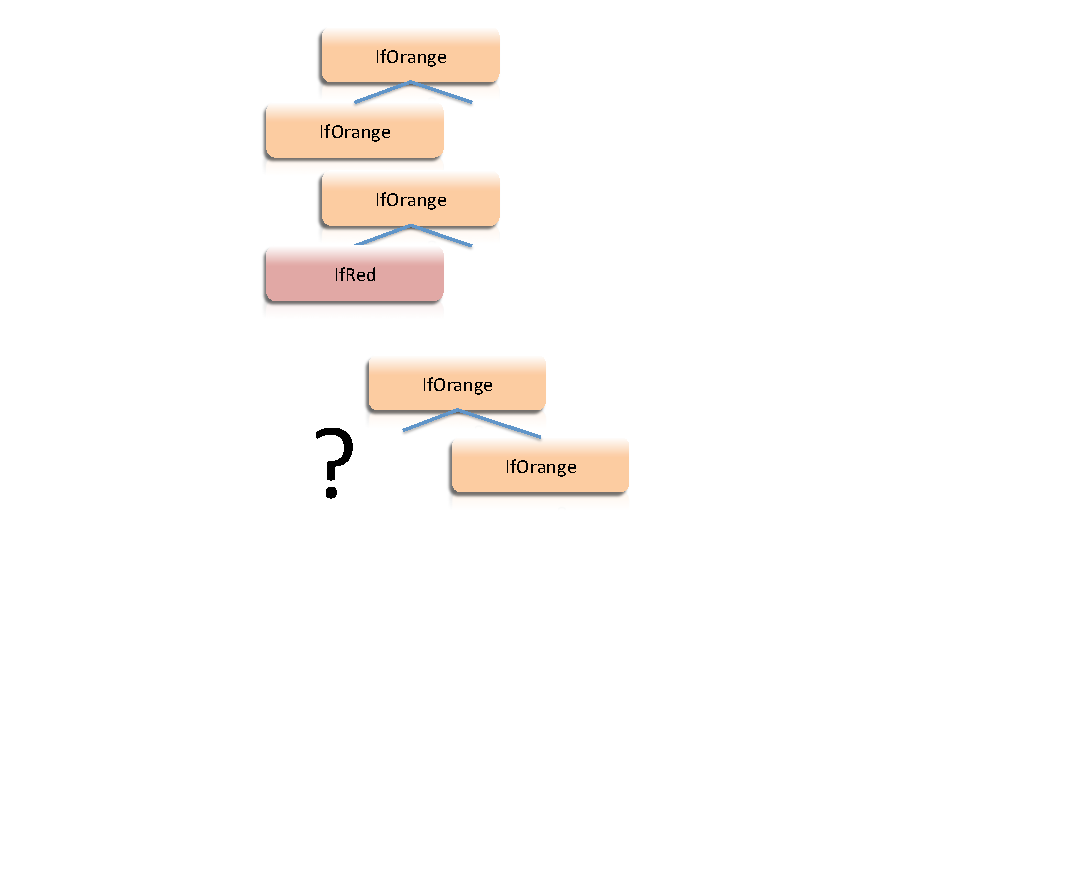
\includegraphics[width=0.45\textwidth]{figs/pdf/leng1ejem2}
\caption{Árboles válidos que carecen de sentido de la solución 1.}
\label{fig:leng1ejemplo2}
\end{figure}


\clearpage


\subsection{Solución 2: Un lenguaje de
funciones y parámetros.}\label{subsec:solucion2}

Uno de los grandes fallos de la solución 1 es que la comprobación del color de
dos casillas diferentes se convierte en un problema en si mismo. Las
comprobaciones deberían poderse hacer en una instrucción sin necesidad de generar
un árbol especifico para encontrar una casilla.

Es por ello que surge la necesidad de un lenguaje fuertemente tipado, donde
existan funciones como test que comprueban en que una casilla seleccionada por
parámetros coincida con el valor del color pasado por parámetros, es decir:
test faceUp x1 y2 colorRed(comprueba que la casilla x1 y2 de la cara de
arriba sea de color rojo). La necesidad de los parámetros se justifica porque si queremos
generar una función por cada combinación de parámetros posibles tendríamos:

\begin{equation}
   6 caras * 3 casillas_x * 3 casillas_y * 6 colores = 324 nodos
\end{equation}

Esto, además de ser un trabajo inmensamente tedioso, es difícilmente escalable y
sólo podría aplicarse al cubo de Rubik.

Por esto mismo, se crearán los distintos terminales necesarios para referirse a
las casillas (X0,X1,X2,Y0,Y1,Y2), para referirse a las caras (FaceUp, FaceFront,
FaceDown, FaceRight, FaceLeft y FaceBack) y para referirse a los colores
(ColorRed, ColorBlue, ColorGreen, ColorWhite, ColorYellow).

Adicionalmente dispondremos de una función test, que comprobará si una casilla
en concreto es de un color determinado. Si lo es, el valor devuelto de la función
será verdadero. Si no, será falso.

También tendremos todo el conjunto de operaciones condicionales como AND, OR y
NOT. La sentencia If ahora tendrá tres hijos, en lugar de dos, como pasaba en el
lenguaje anterior. El primero de los hijos representa la condición a evaluar, el
segundo es la rama del árbol que se ejecutará si la condición es cierta, si no,
se ejecutará la tercera rama del nodo.

De esta forma obtenemos conjunto de nodos terminales y no-terminales descritos
en las tablas \ref{tab:n-terminales-sol2} y \ref{tab:n-noterminales-sol2}
respectivamente (figuras \ref{fig:leng2nodosterm}, 
\ref{fig:leng2nodosnotermaction} y \ref{fig:leng2nodosnotermcond}).

\begin{table}[ctb]
\caption{Tabla de nodos terminales de la solución 2.}
\label{tab:n-terminales-sol2}
\centering
\begin{tabular}{lcp{8cm}}
\toprule
\textbf{Nombre} &\textbf{Tipo}& \textbf{Descripción}\\
\midrule
\textbf{X0}	&XNode&	Se trata de la representación de la posición x0 de una cara
del cubo de Rubik.\\\hline
\textbf{X1}	&XNode&	Se trata de la representación de la posición x1 de
una cara del cubo de Rubik.\\\hline
\textbf{X2}&	XNode&	Se trata de la representación de la
posición x2 de una cara del cubo de Rubik.\\\hline
\textbf{Y0}&	YNode&	Se trata de la
representación de la posición y0 de una cara del cubo de Rubik.\\\hline
\textbf{Y1}&YNode	&Se trata de la representación de la posición y1 de una cara
del cubo de Rubik.\\\hline
\textbf{Y2}&	YNode	&Se trata de la representación de la posición y2 de una cara
del cubo de Rubik.\\\hline
\textbf{FaceLeft}&	FaceNode	&Se trata de la representación de la cara izquierda
del cubo de Rubik.\\\hline
\textbf{FaceUp}&	FaceNode&	Se trata de la representación de la cara superior del
cubo de Rubik.\\\hline
\textbf{FaceFront}&	FaceNode &	Se trata de la representación de la cara frontal
del cubo de Rubik.\\\hline
\textbf{FaceRight}&	FaceNode&	Se trata de la representación de la cara derecha
del cubo de Rubik.\\\hline 
\textbf{FaceDown}&	FaceNode&	Se trata de la representación de la cara inferior
del cubo de Rubik.\\\hline
\textbf{FaceBack}	&FaceNode	&Se trata de la representación de la cara trasera
del cubo de Rubik.\\\hline
\textbf{Red}	&ColorNode&	Se trata de la representación del color rojo del cubo
de Rubik.\\\hline 
\textbf{Orange}&	ColorNode &	Se trata de la representación del color naranja del
cubo de Rubik.\\\hline 
\textbf{Green}	&ColorNode&	Se trata de la representación del color verde del
cubo de Rubik.\\\hline 
\textbf{White}	&ColorNode&	Se trata de la representación del color blanco del
cubo de Rubik.\\\hline 
\textbf{Yellow}&	ColorNode&	Se trata de la representación del color amarillo del
cubo de Rubik.\\\hline 
\textbf{Blue}	&ColorNode&	Se trata de la representación del color azul del cubo
de Rubik.\\\hline 
\textbf{Clockwise}&	DirectionNode&	Es el sentido de rotación de las agujas del
reloj de una cara. \\\hline 
\textbf{CounterClockwise}	&DirectionNode&	Es el sentido de rotación en sentido
contrario a las agujas del reloj de una cara.\\
\bottomrule
\end{tabular}
\end{table}

\begin{table}[ctb]
\caption{Tabla de nodos no-terminales de la solución 2.}
\label{tab:n-noterminales-sol2}
\centering
\begin{tabular}{lccp{8cm}}
\toprule
\textbf{Nombre} &\textbf{Tipo}&\textbf{Aridad}& \textbf{Descripción}\\
\midrule
\textbf{Test}	&CondNode&4&	Comprueba que en la cara especificada (nodo 0), en la
posición especificada (nodo 1 se refiere a x  y nodo 2 se refiere a  y) sea del color especificado (nodo 3).\\\hline 
\textbf{And}	&CondNode&2&Realiza la operación booleana AND entre sus dos
hijos.\\\hline
\textbf{Or}	&CondNode&2&Realiza la operación booleana OR entre sus dos
hijos.\\\hline \textbf{No}	&CondNode&1&Realiza la operación booleana NOT de su hijo.\\\hline 
\textbf{Move}	&ActionNode&2&Mueve la cara (nodo 0) en la dirección (nodo 1)
especificado.\\\hline 
\textbf{If}	&ActionNode&3&	Comprueba que la condición especificada en el hijo 0
se cumpla. Si se cumple ejecuta el subárbol del hijo 1, si no, el subárbol 2.\\\hline 
\textbf{Progn2}	&ActionNode&2&	Ejecuta todos sus hijos.\\\hline 
\textbf{Progn3}	&ActionNode&3&	Ejecuta todos sus hijos.\\
\bottomrule
\end{tabular}
\end{table}

\begin{figure}[t]
\centering
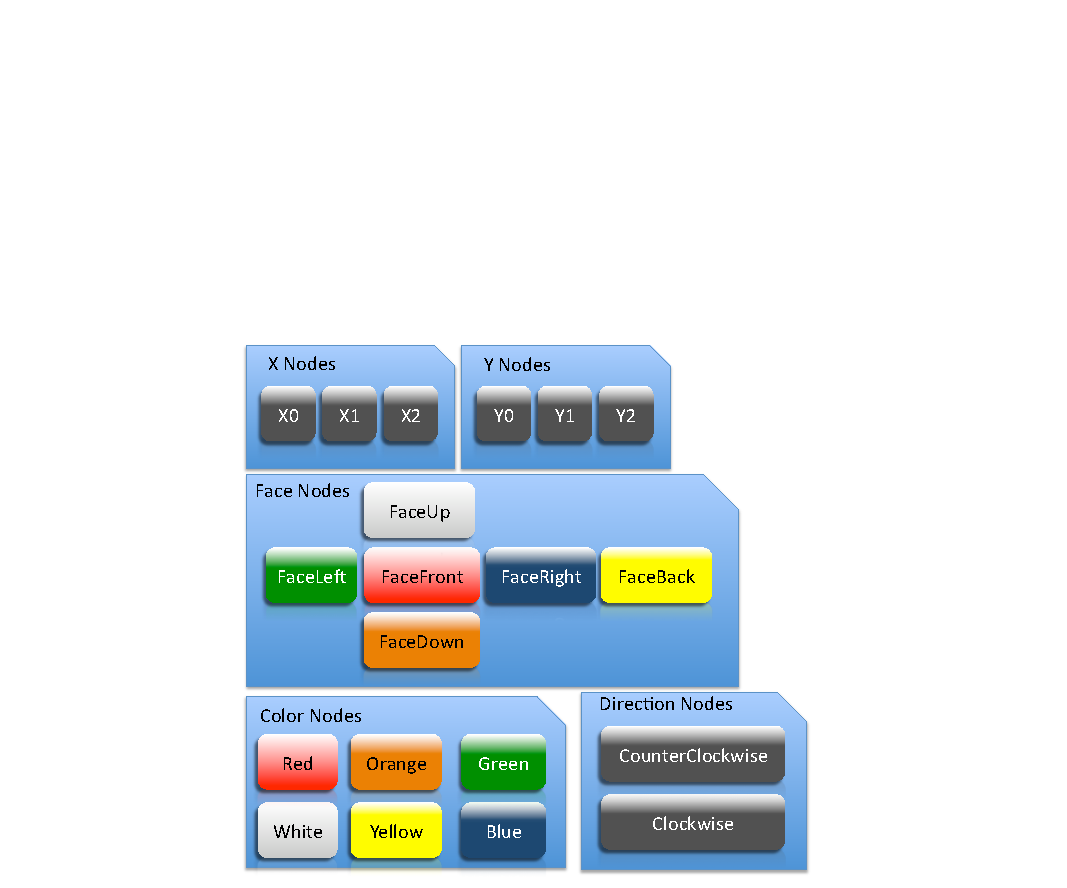
\includegraphics[width=0.65\textwidth]{figs/pdf/leng2nodosterm}
\caption{Nodos terminales de la solución 2.}
\label{fig:leng2nodosterm}
\end{figure}

\begin{figure}[t]
\centering
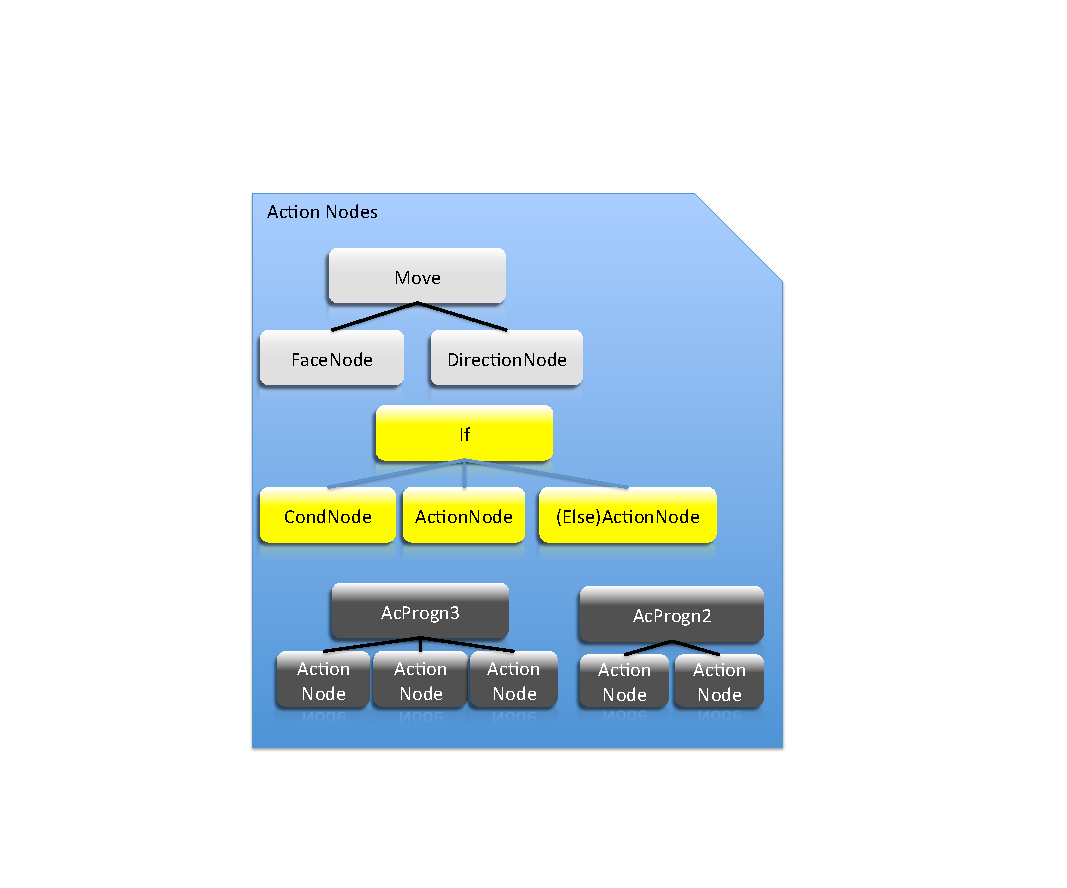
\includegraphics[width=0.65\textwidth]{figs/pdf/leng2nodosnotermaction}
\caption{Nodos no terminales de la solución 2.}
\label{fig:leng2nodosnotermaction}
\end{figure}

\begin{figure}[t]
\centering
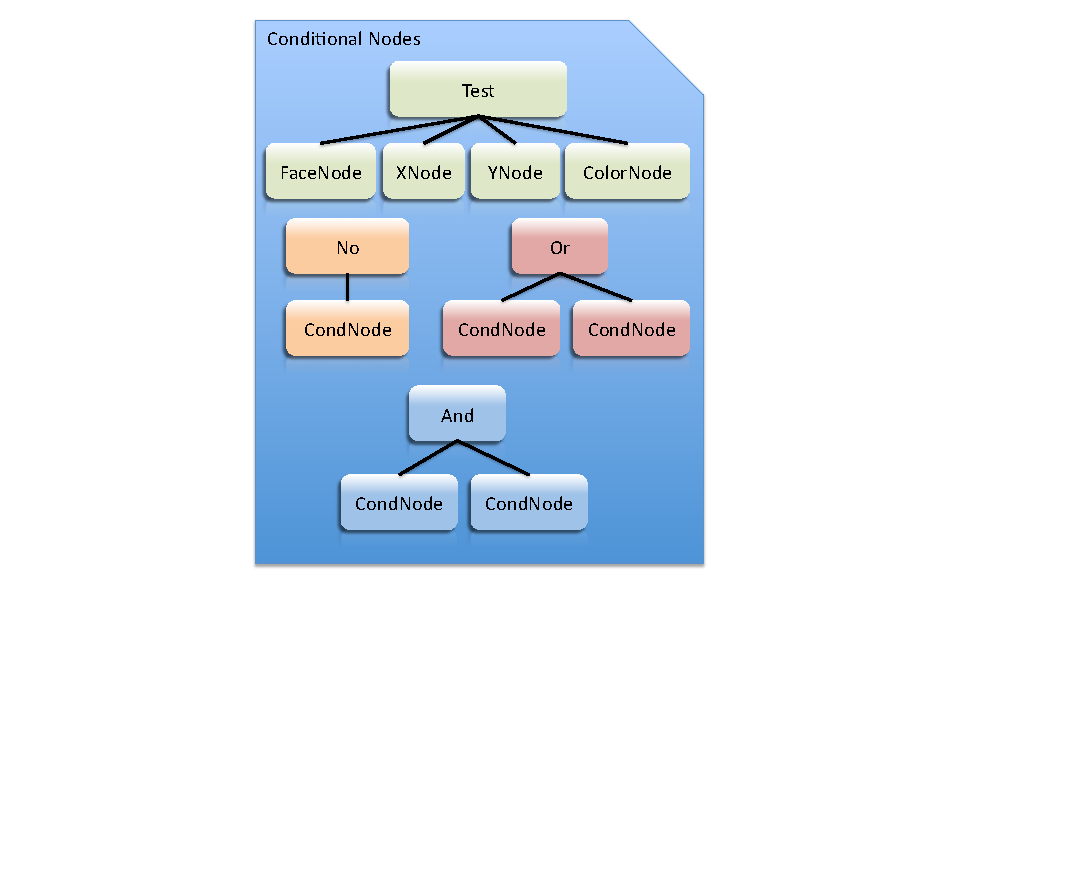
\includegraphics[width=0.65\textwidth]{figs/pdf/leng2nodosnotermcond}
\caption{Nodos no terminales de la solución 2.}
\label{fig:leng2nodosnotermcond}
\end{figure}


A diferencia con el lenguaje anterior, en este lenguaje cualquier nodo no es
compatible con otro. Por lo tanto, que la operación de cruzamiento puede que
resulte mucho más costosa y requiera de muchos más intentos para que se pueda
producir. Cuando el operador de cruzamiento ha agotado todos sus intentos de
buscar una combinación correcta del código genético, la consecuencia resultante
aparece como la copia del individuo en la nueva población. Este suceso no aporta
nada nuevo a la siguiente generación, y, por lo tanto, si no configuramos
correctamente el algoritmo, la evolución se verá comprometida.

Sin embargo, las ventajas de este lenguaje son enormes. La complejidad a la hora
de comprobar el estado del cubo ha disminuido enormemente, de tal forma que ya no
constituye un problema en si mismo. Antes, en el peor de los casos eran
necesarios nueve pasos para llegar a la casilla más distante y comprobar su
color. Ahora solo se requiere un paso. Además, las expresiones condicionales
pueden expresar situaciones mucho más complejas ya que ahora es posible utilizar
operadores como AND, OR y NO.

Para resolver el ejemplo propuesto en la solución anterior (figura
\ref{fig:leng2ejem1}) necesitaríamos de los siguientes operadores: 

\begin{algorithmic}
\IF {($Test$ $FaceUp$ $X0$ $Y0$ $Red$) $AND$ ($Test$ $FaceFront$ $X1$ $Y0$
$Red$)} 
	\STATE $Move$ $FaceLeft$ $Clockwise$
\ENDIF 
\end{algorithmic}
. Como se puede observar, la sentencia es mucho mas
simple y por otra parte, mucho más fácil de entender.

En conclusión, aunque hemos dado con un lenguaje bastante apropiado para
representar la solución del problema, necesitamos explotar la potencia de este
lenguaje. Con el árbol que hemos expuesto anteriormente sólo somos capaces de
resolver 1 caso de los 12 posibles de nivel 1 (figura \ref{fig:leng2ejem2}), lo
que resulta en unas estadísticas muy poco favorables para la complejidad del árbol. Sin duda podemos
sacar más información del árbol de programa expuesto. El siguiente lenguaje que
veremos explotará al máximo las posibilidades del este lenguaje.




\begin{figure}[t]
\centering
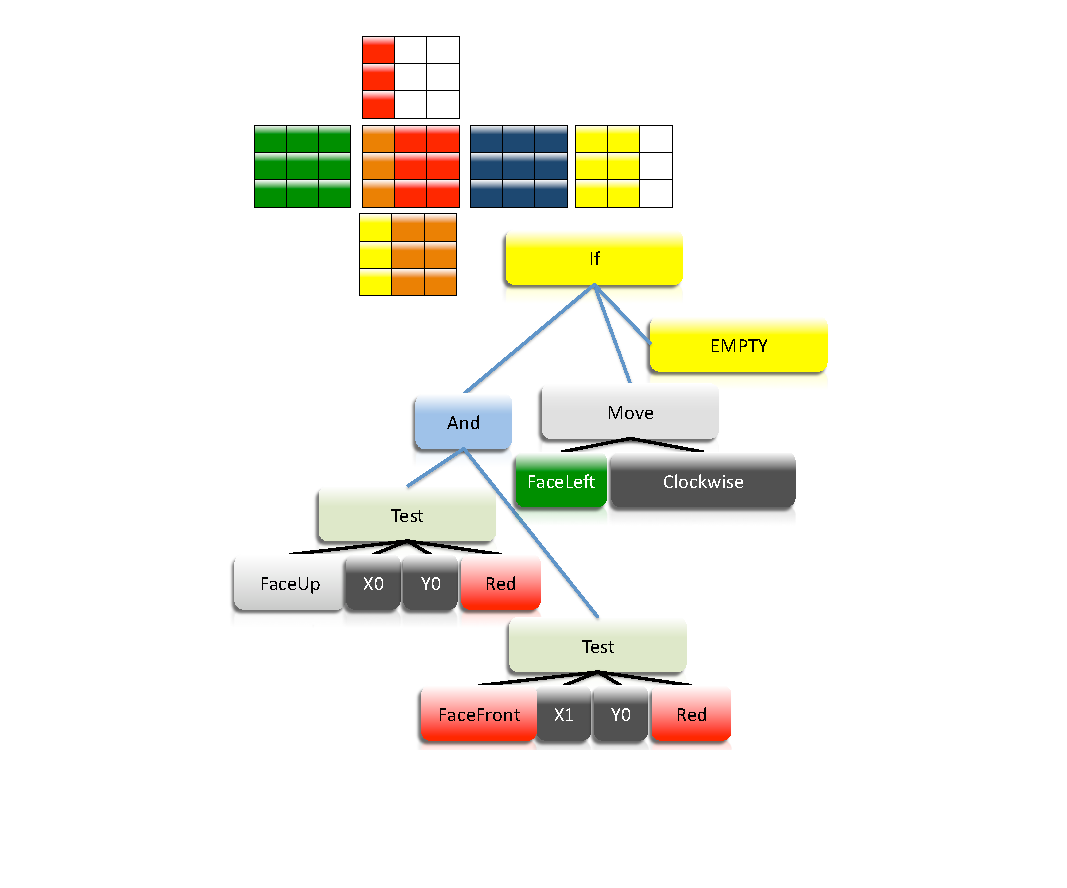
\includegraphics[width=0.65\textwidth]{figs/pdf/leng2ejem1}
\caption{Ejemplo de árbol de la solución 2 que resuelve un cubo de rubik de
nivel 1.}
\label{fig:leng2ejem1}
\end{figure}

\begin{figure}[t]
\centering
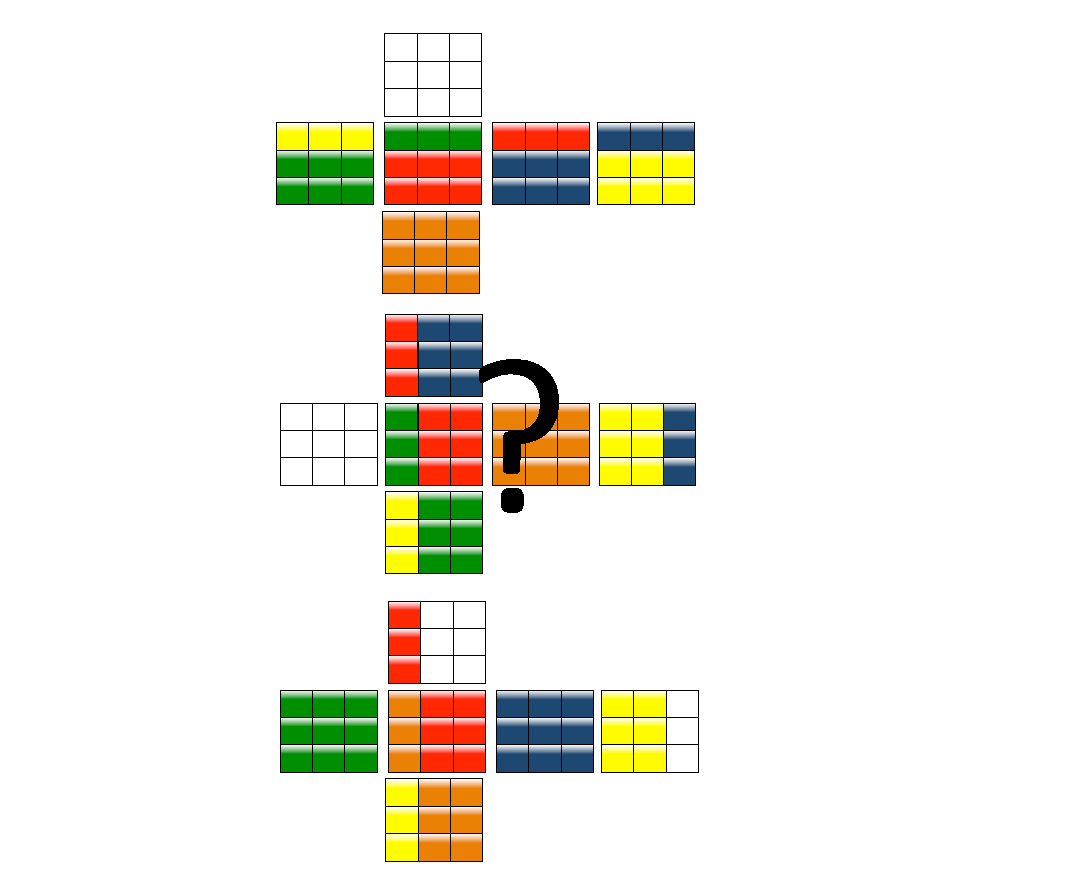
\includegraphics[width=0.45\textwidth]{figs/pdf/leng2ejem2}
\caption{Cubos de estado similar.}
\label{fig:leng2ejem2}
\end{figure}

\clearpage


\subsection{Solución 3: La abstracción del cubo.}\label{subsec:solucion3}

Una de las características del cubo de Rubik es que existen estados que son
equivalentes, simétricos: existe una serie de rotaciones del conjunto completo
que transforman un estado en otro. Nuestro cerebro es capaz de abstraer todos
estos estados y unificarlos en solo estado y por lo tanto, un camino de
resolución posible. Por otro lado, también es capaz de abstraer los colores
específicos del cubo de Rubik, y puede trabajar en la misma situación con colores
diferentes sin necesidad de adaptación alguna.

Pongamos un ejemplo. Para todos los cubos de nivel 1, es decir, con un solo
desplazamiento de la solución, nuestro cerebro solo ve dos estados diferentes y
por lo tanto dos soluciones. Estos dos casos surgen de mover cualquier cara en el
sentido de las agujas del reloj, el primero y el segundo cuando movemos una cara
en sentido opuesto a las agujas del reloj. De esta forma se podrían reducir los
12 primeros casos, en dos simples casos: cuándo debo girar en el sentido de las
agujas del reloj y cuando no.

Para imitar este comportamiento y adaptarlo a nuestro sistema se han realizado
dos modificaciones importantes sobre el segundo lenguaje.

La primera es que los colores ya no son colores concretos, como rojo o verde,
sino abstracciones como color1 o color2 que pueden tomar diferentes valores en
momentos concretos. Así en color1 puede referirse al color rojo en un momento
determinado, y luego puede referirse al verde. Una situación que no puede ocurrir
es que el color 1 se refiera al verde y el color 2 también. El color 1 es
diferente al color 2.

La segunda de estas modificaciones refleja la segunda parte del proceso de
abstracción. Para conseguirlo, el cubo será rotado en todas sus posibilidades
para cubrir todos los estados equivalentes, mientras se verifica si en alguna de
esas rotaciones se cumple la condición expuesta. Si se cumple el sistema de
rotaciones parará y dejará el cubo preparado para recibir los movimientos
pertinentes en función de la condición especificada.

Estas dos modificaciones las llevará a cabo la sentencia If y Test. If se
encargará de rotar el cubo hasta que su condición se cumpla. Si no se cumple no
se ejecutará el subárbol de acción. Además desaparece el subárbol else ya que no
tiene sentido sin un previo If que coloque el cubo en la posición adecuada.

Test se encargará de la asignación de los colores. Comprobará si existe alguna
asignación anterior al color que se quiere comprobar. Si no existe, devolverá
verdadero y asignará el color especifico al color abstracto (color 1 = red). Si
el color esta ya asignado, entonces, el color abstracto tomará ese valor. Si el
color que existe en esta posición no coincide con el color especificado, entonces
se devolverá false.

Cuando una condición no se cumple, la función If desasigna todos los colores
abstractos, rota el cubo y vuelve a empezar de nuevo, comprobando que se cumpla
la condición que anida. Una vez que se ha encontrado una forma de que la
condición se cumpla, se dejará en posición deseada el cubo de Rubik para que el
grupo de acciones que vienen a continuación actúen sobre el cubo.

Una vez planteadas las modificaciones del lenguaje se procede a describir todos 
sus nodos empezando por el grupo de terminales (tabla
\ref{tab:n-terminales-sol3}) y el grupo de terminales (tabla
\ref{tab:n-noterminales-sol3}) (figuras \ref{fig:leng3nodosterm},
\ref{fig:leng3nodosnoterma} y \ref{fig:leng3nodosnotermb}).

\begin{table}[ctb]
\caption{Tabla de nodos terminales de la solución 3.}
\label{tab:n-terminales-sol3}
\centering
\begin{tabular}{lcp{8cm}}
\toprule
\textbf{Nombre} &\textbf{Tipo}& \textbf{Descripción}\\
\midrule
\textbf{X0}&	XNode&	Se trata de la representación de la posición x0 de una cara
del cubo de Rubik.\\\hline
\textbf{X1}&	XNode&	Se trata de la representación de la posición x1 de
una cara del cubo de Rubik.\\\hline
\textbf{X2}&	XNode&	Se trata de la representación de
la posición x2 de una cara del cubo de Rubik.\\\hline
\textbf{Y0}&	YNode&	Se trata de la
representación de la posición y0 de una cara del cubo de Rubik.\\\hline
\textbf{Y1}& YNode&	Se trata de la representación de la posición y1 de una cara
del cubo de Rubik. \\\hline
\textbf{Y2}&	YNode&	Se trata de la representación de la posición y2 de
una cara del cubo de Rubik. \\\hline
\textbf{FaceLeft}&	FaceNode&	Se trata de la
representación de la cara izquierda del cubo de Rubik.\\\hline
\textbf{FaceUp}&	FaceNode&
Se trata de la representación de la cara superior del cubo de Rubik.\\\hline
\textbf{FaceFront}&	FaceNode &	Se trata de la representación de la cara frontal
del cubo de Rubik.\\\hline
\textbf{FaceRight}&	FaceNode&	Se trata de la representación de la cara derecha
del cubo de Rubik.\\\hline
\textbf{FaceDown}&	FaceNode&	Se trata de la representación de la cara inferior
del cubo de Rubik.\\\hline
\textbf{FaceBack}&	FaceNode&	Se trata de la representación de la cara trasera
del cubo de Rubik.\\\hline
\textbf{Color1}&	ColorNode	&Se trata de la abstracción de un color del cubo de
Rubik.\\\hline
\textbf{Color2}&	ColorNode &	Se trata de la abstracción de un color del cubo de
Rubik.\\\hline
\textbf{Color3}&	ColorNode&	Se trata de la abstracción de un color del cubo de
Rubik.\\\hline
\textbf{Color4}&	ColorNode&	Se trata de la abstracción de un color del cubo de
Rubik. \\\hline
\textbf{Color5}&	ColorNode&	Se trata de la abstracción de un color del cubo de
Rubik.\\\hline
\textbf{Color6}&	ColorNode&	Se trata de la abstracción de un color del
cubo de Rubik.\\\hline
\textbf{Clockwise}&	DirectionNode&	Es el sentido de rotación de
las agujas del reloj de una cara.\\\hline
\textbf{CounterClockwise}&	DirectionNode&	Es el
sentido de rotación en sentido contrario a las agujas del reloj de una
cara.\\
\bottomrule
\end{tabular}
\end{table}

\begin{table}[ctb]
\caption{Tabla de nodos no-terminales de la solución 3.}
\label{tab:n-noterminales-sol3}
\centering
\begin{tabular}{lccp{8cm}}
\toprule
\textbf{Nombre} &\textbf{Tipo}&\textbf{Aridad}& \textbf{Descripción}\\
\midrule
\textbf{Test}&CondNode&	4	&Comprueba que en la cara especificada (nodo 0), en la
posición especificada (nodo 1 se refiere a x  y nodo 2 se refiere a  y) sea del
color especificado (nodo 3).\\\hline
\textbf{And}&	CondNode&	2&	Realiza la operación booleanas AND entre sus dos
hijos.\\\hline 
\textbf{Or}&	CondNode&	2&	Realiza la operación booleana OR entre sus
dos hijos.\\\hline
\textbf{No}& CondNode&	1&	Realiza la operación booleana NOT de su
hijo.\\\hline
\textbf{If}&IfNode&	2&	Se
trata de la representación de la posición y2 de una cara del cubo de
Rubik.\\\hline
\textbf{Progn2}&	IfNode	&2&	Ejecuta todos sus hijos.\\\hline
\textbf{Progn3}&	IfNode	&3&	Ejecuta todos sus hijos.\\\hline
\textbf{Move}	&ActionNode	&2&	Mueve la cara (nodo 0) en la dirección (nodo 1)
especificado.\\\hline
\textbf{Progn2}&	ActionNode	&2&	Ejecuta todos sus hijos.\\\hline
\textbf{Progn3}&	ActionNode	&3&	Ejecuta todos sus hijos.\\
\bottomrule
\end{tabular}
\end{table}

\begin{figure}[ctb]
\centering
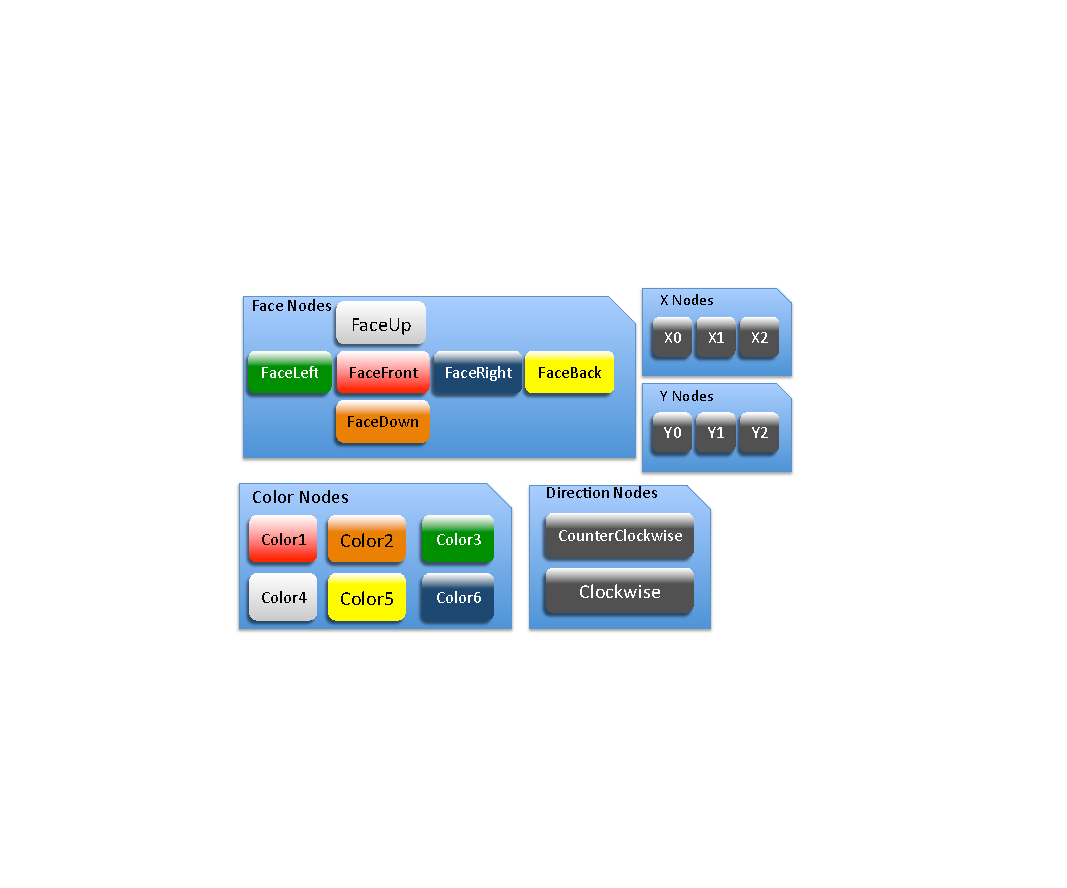
\includegraphics[width=0.65\textwidth]{figs/pdf/leng3nodosterm}
\caption{Nodos terminales de la solución 3.}
\label{fig:leng3nodosterm}
\end{figure}

\begin{figure}[ctb]
\centering
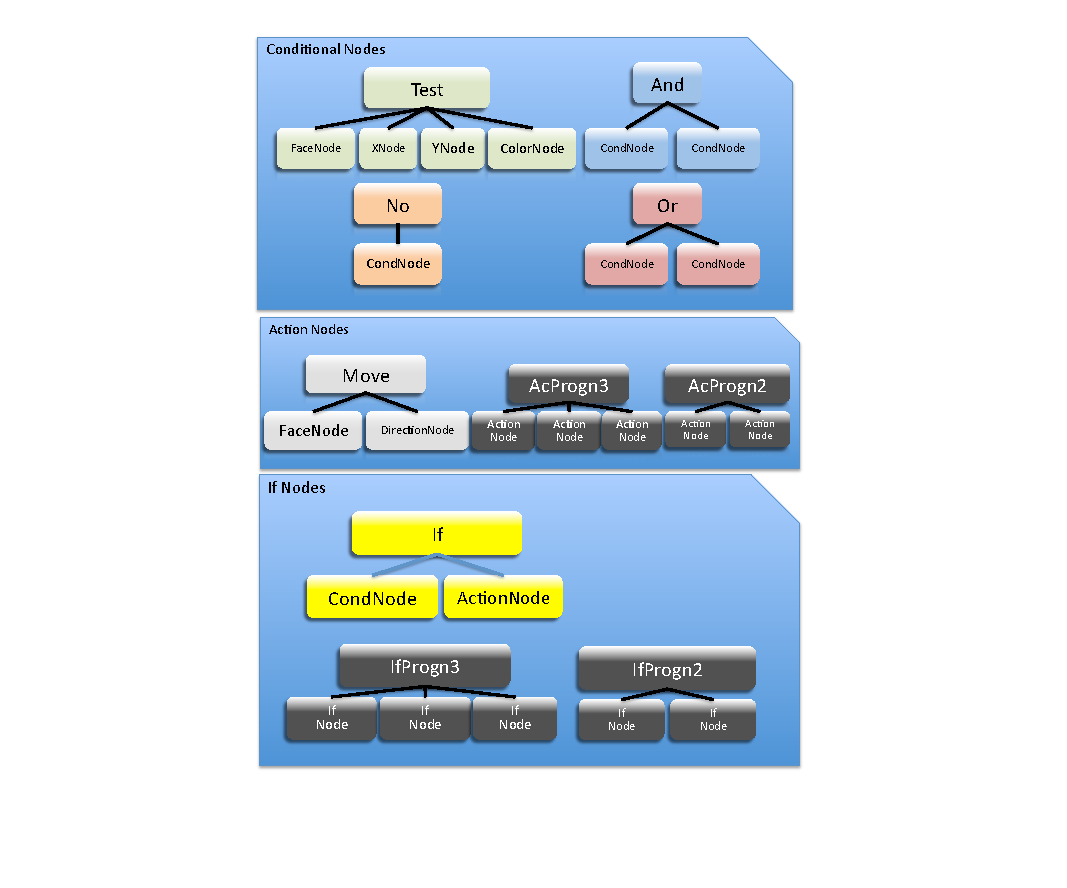
\includegraphics[width=0.65\textwidth]{figs/pdf/leng3nodosnoterma}
\caption{Nodos no terminales de la solución 3.}
\label{fig:leng3nodosnoterma}
\end{figure}

\begin{figure}[ctb]
\centering
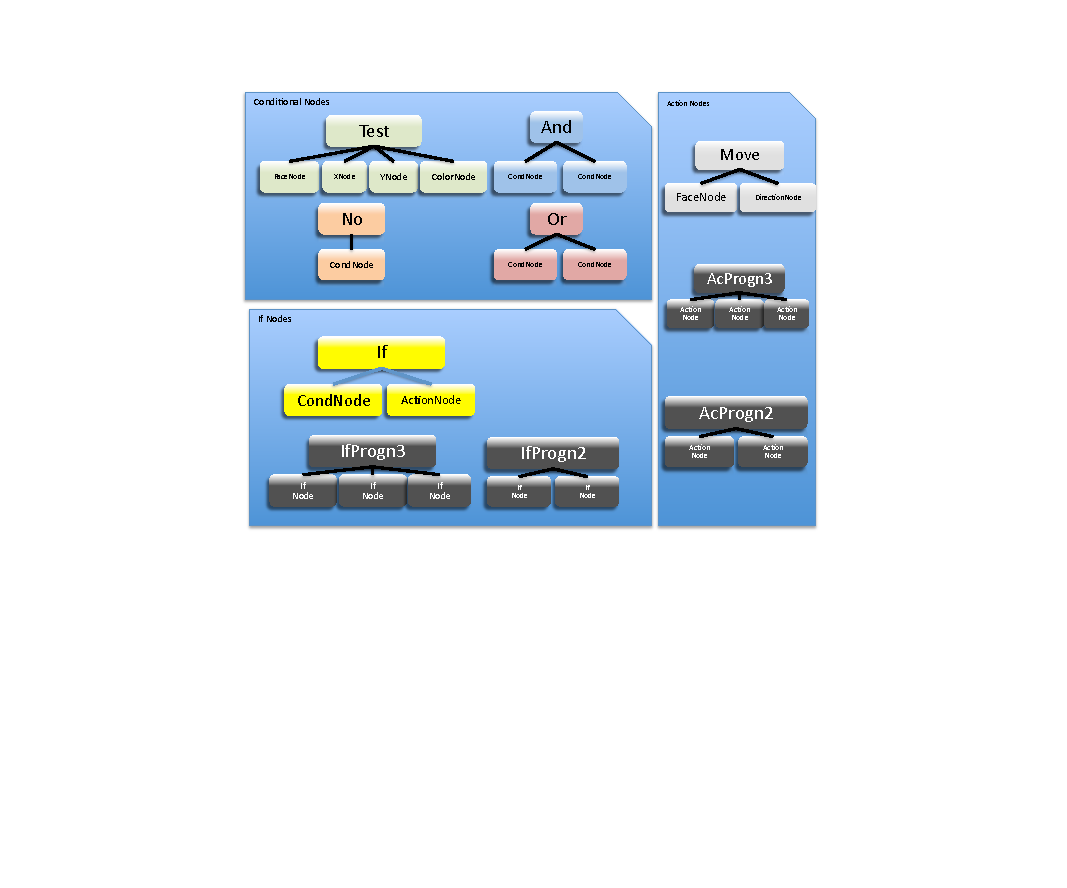
\includegraphics[width=0.65\textwidth]{figs/pdf/leng3nodosnotermb}
\caption{Nodos no terminales de la solución 3.}
\label{fig:leng3nodosnotermb}
\end{figure}

Este lenguaje presenta los mismo síntomas y problemas que aparecían en el 
anterior con la diferencia de que el nodo If no contiene Else. Además, la
anidación de sentencias If deja de tener sentido por lo que nuestro programa
pasará a ser una “lista” de sentencias If ya que los operadores de movimiento no
tienen sentido si no existen un If que lo contenga.

Las ventajas son claras y evidentes. Donde antes resolvíamos dos cubos de Rubik,
ahora resolvemos doce (figuras \ref{fig:leng3ejem1} y \ref{fig:leng3ejem2}). Es
decir, nuestro lenguaje resulta mucho más potente. Otro factor a tener en cuenta es que al ser un lenguaje altamente tipado el bloat que
se puede producir es menor.




\begin{figure}[t]
\centering
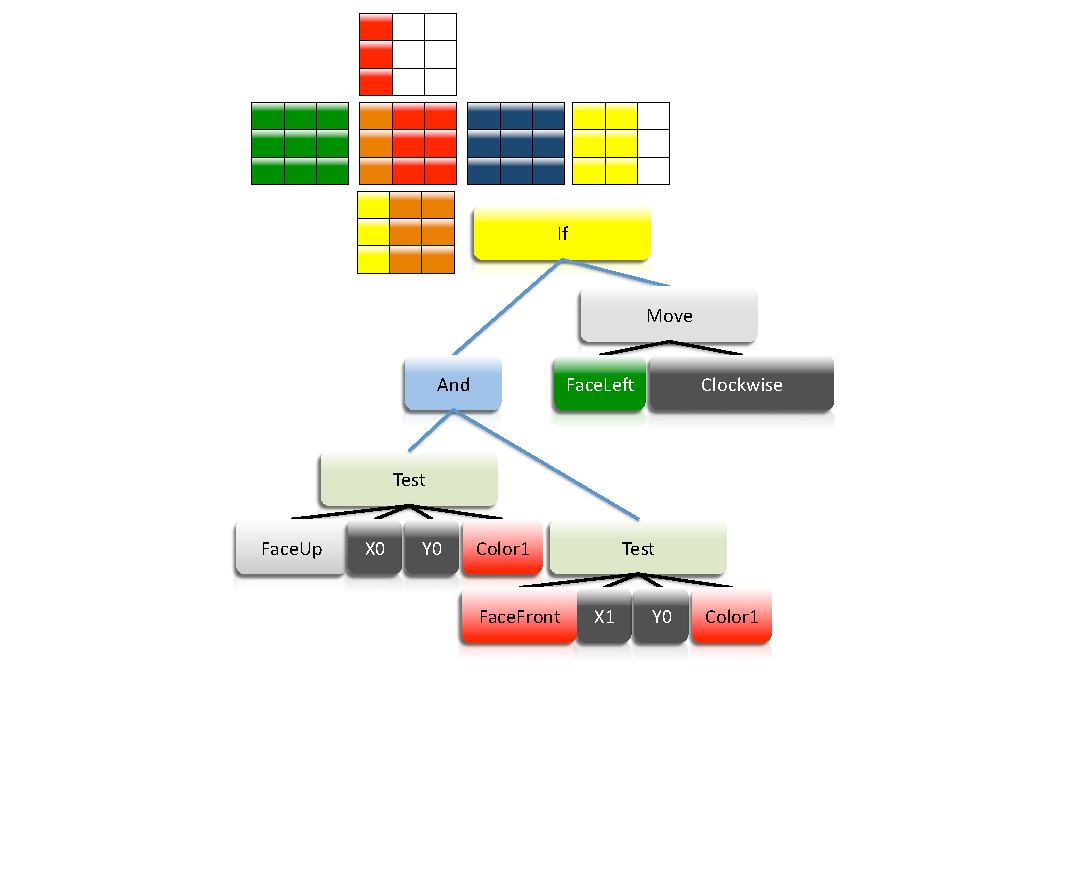
\includegraphics[width=0.65\textwidth]{figs/pdf/leng3ejem1}
\caption{Ejemplo de árbol de la solución 3 que resuelve un cubo de rubik de nivel 1.}
\label{fig:leng3ejem1}
\end{figure}

\begin{figure}[t]
\centering
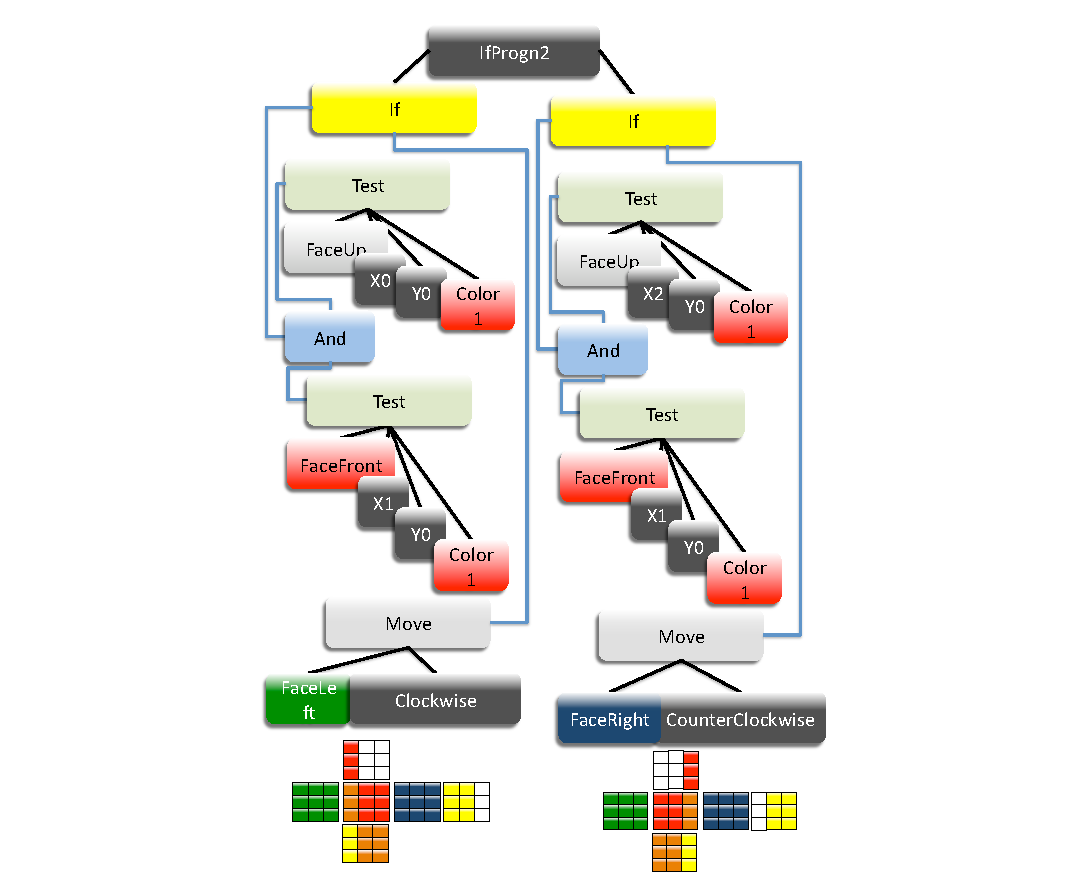
\includegraphics[width=0.9\textwidth]{figs/pdf/leng3ejem2}
\caption{Árbol que resuelve todos los cubos de rubik de nivel 1.}
\label{fig:leng3ejem2}
\end{figure}

\clearpage

\section{Fitness}\label{sec:fitness}


El fitness es una nota o un conjunto de calificaciones o notas de un programa que
sirven para decidir cuando un programa es mejor que otro. En nuestro caso
necesitamos varias medidas de fitness. Necesitamos un valor que nos indique lo
cerca de la solución que un programa deja a los cubos. De esta forma, un programa
será mejor cuanto más cerca de la solución deje el cubo. A esta puntuación se la
llamará entropía, descrita en el siguiente punto.

No obstante, cuando tenemos varios cubos en juego podemos obtener más información
sobre el rendimiento del algoritmo. Por ejemplo podremos saber cuántos cubos
resuelve un programa. Es más, ya que tenemos una manera de clasificar los cubos
mediante sus dificultades, podemos sesgar la búsqueda y guiar a los programas
para que primen los cubos difíciles respecto a los más fáciles.

Otro dato que necesitamos saber es la longitud de las soluciones. Ya que nos
conviene encontrar el camino óptimo, necesitamos saber el tamaño de la solución
para poder elegir el programa que menor longitud de solución tenga.

Por último, para controlar el bloat producido, podremos considerar en el fitness
el número de nodos que posee el programa, ya que si encontramos un programa que
hace lo mismo con menos código puede sernos de interés.

Al final del proceso, cuando estamos comparando dos programas, uno tiene que
inclinarse a por elegir uno u otro. Para ello necesitaremos comparar y unir de
alguna forma todos estos objetivos en un objetivo común. De esto hablaremos en el
último punto de este apartado. 

\subsection{Entropía}\label{subsec:entropia}

La razón de esta medición es que nos interesa saber cuánto de cerca estamos de
solventar el cubo de Rubik. Podríamos obtener este dato mediante la utilización
de algoritmos de resolución del cubo de Rubik existentes. No obstante, estos
algoritmos utilizan muchos recursos y multiplicando éstos por cada individuo de
la población resultaría una utilización inviable de los recursos y la potencia de
cálculo del sistema. Por otro lado necesitamos un criterio ajeno a cualquier
sistema de búsqueda preexistente para no predeterminar a los individuos. Por lo
tanto hemos desarrollado un método basado en la entropía del cubo que nos dirá
con más o menos acierto lo cerca que estamos de una solución.

\begin{figure}[t]
\centering
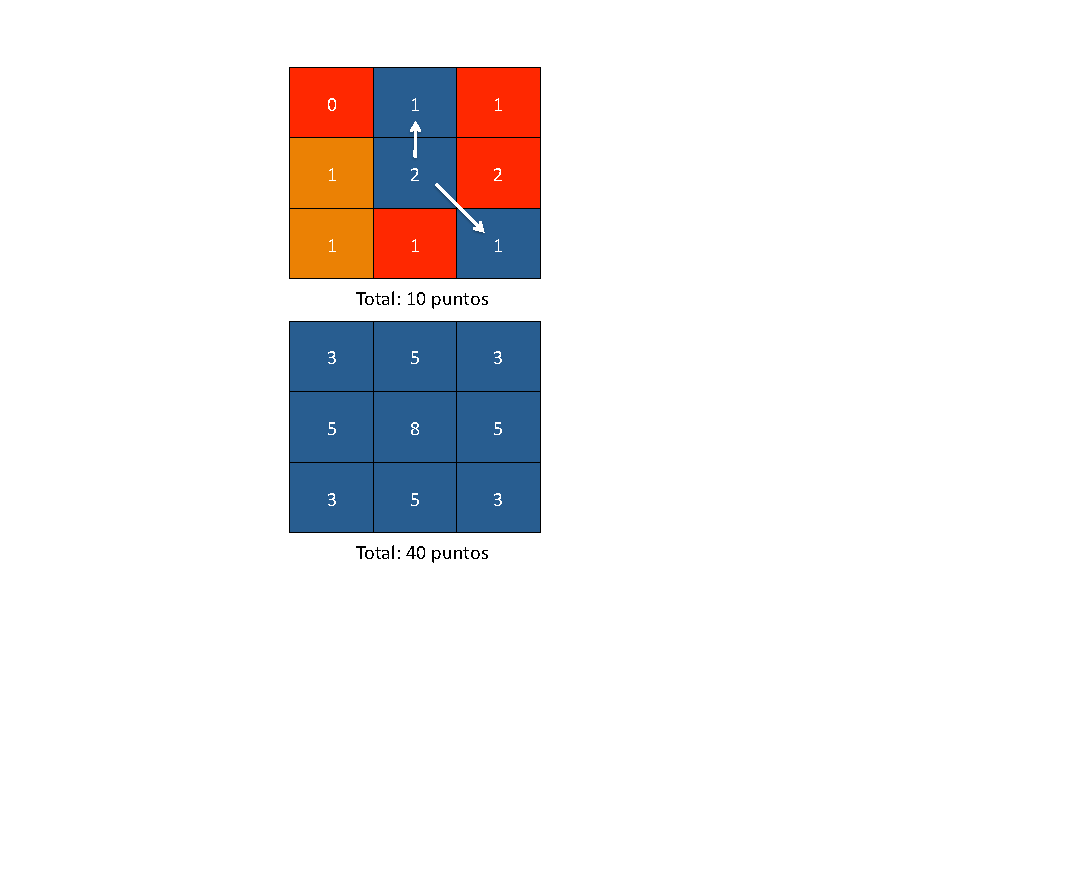
\includegraphics[width=0.35\textwidth]{figs/pdf/entropia}
\caption{Entropía.}
\label{fig:entropia}
\end{figure}

El cálculo de la entropía del cubo consiste en la suma de las casillas del mismo
color que estén contiguas dentro de una misma cara. Es decir, sumamos un punto
por cada casilla que esté contigua dentro de la misma cara y que sea del mismo
color. Por consiguiente, una cara resuelta sumaría 40 puntos
(figura \ref{fig:entropia}), y entonces un cubo de Rubik resuelto sumaría 240
puntos.

El pseudocódigo del algoritmo sería el siguiente:


\begin{algorithmic}
\FOR{each cara}
	\STATE puntuacionCara = $0$
	\FOR{each casilla}
		\IF {CasillaArriba.color == CasillaActual.color}  
				\STATE puntuacionCara++
		\ENDIF
		\IF {CasillaArribaIzq.color == CasillaActual.color}  
				\STATE puntuacionCara++
		\ENDIF
		\IF {CasillaIzquierda.color == CasillaActual.color}  
				\STATE puntuacionCara++
		\ENDIF
		\IF {CasillaAbajoIzq.color == CasillaActual.color}  
				\STATE puntuacionCara++
		\ENDIF
		\IF {CasillaAbajo.color == CasillaActual.color}  
				\STATE puntuacionCara++
		\ENDIF
		\IF {CasillaAbajoDer.color == CasillaActual.color}  
				\STATE puntuacionCara++
		\ENDIF
		\IF {CasillaDerecha.color == CasillaActual.color}  
				\STATE puntuacionCara++
		\ENDIF
		\IF {CasillaArribaDer.color == CasillaActual.color}  
				\STATE puntuacionCara++
		\ENDIF
	\ENDFOR 
	\STATE puntuacionTotal += puntuacionCara
\ENDFOR 
\end{algorithmic}

Con este método es posible encontrar estados intermedios más cercanos a la meta
que posean menor entropía. Sin embargo, la tendencia general del cubo es a
aumentar el orden de las casillas según se acerque a la solución. Además, esta
medida se utilizará para comparar el estado final del cubo finalizada la
ejecución de un programa frente al estado final del mismo cubo finalizada la
ejecución de otro programa, por lo tanto, esta nota no servirá para evaluar
estados intermedios sino sólo los finales.
 
\subsection{Cubos resueltos}\label{subsec:cubosresueltos}

Una vez que conseguimos resolver cubos, es trivial comparar programas en función
del número de cubo que resuelve uno y el número de cubos de Rubik que resuelve
otro. Sin embargo, podemos explotar esta medición incorporando nuevos parámetros,
como es la dificultad de los cubos resueltos.

Al generar los primeros programas podemos ver en las estadísticas que existen muy
pocos de ellos que puedan resolver un cubo de alta dificultad. Sin embargo, de
los programas generados por el algoritmo genético hay muchos más que pueden
resolver cubos fáciles. Y esos programas que resuelven cubos fáciles son, además,
capaces de resolver muchas clases de cubos fáciles. Por el contrario, los
programas resolvedores de cubos difíciles sólo son capaces de resolver un número
muy limitado de dichos cubos.

Como el algoritmo selecciona los programas que más cubos resuelven, los
resolvedores de cubos difíciles van desapareciendo, de tal forma que sólo
sobreviven los programas capaces de resolver los cubos fáciles. Esto hace que
disminuya enormemente la diversidad genética de nuestro sistema. En definitiva
necesitamos buscar alguna forma de calibrar el fitness para mantener con vida a
los individuos que pueden resolver cubos difíciles.

Así, necesitamos premiar de alguna forma a los programas que resuelven cubos
difíciles. Una alternativa sería realizar una suma ponderada linealmente de los
cubos resueltos de cada dificultad. Sin embargo la ponderación lineal no pondera
lo suficiente ya que, es fácil encontrar un programa que resuelva más cubos de
dificultad fácil que de la dificultad estrictamente superior. Esto es debido a
que por cada nivel aparecen doce nuevas posibilidades, por lo que, resolver el
siguiente nivel resulta doce veces más difícil. Es por esto que necesitamos una
ponderación exponencial.

Sin embargo en la ponderación necesitamos encontrar un factor que regule la suma
de los cubos resueltos de diferentes niveles. La forma de encontrar este valor
será de forma empírica, buscando el valor que obtenga el mejor rendimiento de la
evolución. Para ello la base de la potencia será configurable mediante parámetros
del algoritmo.

La fórmula
\begin{equation}
   p = c*f ^ d,
\end{equation}
es la fórmula del fitness donde $p$ es la puntuación del programa, $c$ son los
cubos resueltos por el programa, $f$ es el factor elegido y $d$ es la
dificultad de los cubos resueltos.
 

La puntuación final del programa será la suma de las multiplicaciones del número
de cubos resueltos de una dificultad por un factor elevado a la dificultad del
cubo resuelto.


\subsection{Longitud de la solución}\label{subsec:long-solucion}


Para poder controlar la longitud de las soluciones de los cubos que genera un
programa es necesario tener en cuenta este hecho en el fitness. Calcular las
longitudes de las soluciones de los programas es un proceso muy sencillo. Lo
único que requiere es un contador que se inicializa a cero antes de intentar
resolver cualquier cubo de Rubik. Posteriormente, en cada ocasión que se rota una
cara de un cubo se sumará una unidad a este contador. Una vez que la ejecución
del árbol de programa ha terminado, es decir, el programa ha terminado de
intentar resolver el cubo en cuestión, se guardará el número de pasos realizados
por el programa para este cubo. Este proceso se repetirá por cada cubo de Rubik a
resolver.

Cuando el programa termine de intentar resolver todos los cubos de Rubik que le
han sido asignados en el proceso de evaluación, se calculará la media del número
de pasos alcanzado en cada cubo. En base a esa media podremos determinar que
programa es capaz de generar soluciones generalmente más cortas.

\subsection{Bloat}\label{subsec:bloat}

El bloat es el código que se genera dentro los programas evolucionados que carece
de sentido. Como la evolución es un proceso aleatorio, no se encarga de verificar
si el código que se genera tiene sentido o no tiene sentido. Es por ello que
tenemos que realizar esta comprobación de forma manual. Para ello lo único que
tenemos que hacer es calcular el número de nodos que hay en nuestro sistema. Esto
se hace utilizando un simple algoritmo recursivo que recorre todos los nodos del
árbol del programa, contando uno por cada nodo que pasa.

Una vez que tenemos esta función, podremos decir que un programa será mejor
cuando tenga menos nodos que otro programa, es decir, contenga menos
instrucciones.

\subsection{Combinación del fitness}\label{subsec:combinacion-fitness}

Una vez que tenemos preparados numéricamente todos los objetivos necesitaremos
crear un criterio de unión para fusionar todas las calificaciones de un programa.
Como hemos visto en el apartado del estado del arte, existen multitud de maneras
de combinar todos estos objetivos. Nosotros hemos escogido utilizar una política
de prioridades, es decir, definimos la existencia de calificaciones que
prevalecen sobre otras, y sólo cuando las calificaciones de nivel superior son
iguales en ambos programas, el resto de calificaciones serán estudiadas en mas
detalle.

Hemos optado por esta política ya que hemos comprobado que el hacer un control
del bloat demasiado exhaustivo durante la propia evolución puede impedir que ella
misma tenga lugar, por lo que para no tener problemas, sólo se utilizará cuando
consigamos resolver todos los cubos de Rubik.

El mismo efecto que el bloat tiene el número de pasos. Como es obvio, no mover
nada en el cubo de Rubik tiene menos pasos que mover algo. Como nuestro primer
objetivo es conseguir resolver todos los cubos de Rubik, necesitamos que el
sistema mueva las caras. Por lo tanto, esta calificación tampoco se tendrá en
cuenta hasta que se hayan resuelto todos los cubos propuestos en la evaluación.

La entropía nos valdrá para deqcidir qué programa es mejor que otro cuando exista
un empate numérico de la puntuación de cubos resueltos. Esto se justifica en que
cuando dos programas consiguen resolver el mismo número de cubos, el programa que
mas se acerque a la solución, más cerca estará de resolver un cubo de Rubik y por
lo tanto, de mejorar la puntuación de cubos resueltos.

Como adelantaba, la puntuación principal será la de los cubos resueltos expuesta
en la sección \ref{subsec:cubosresueltos}. Esto es debido a que el objetivo
principal es resolver los cubos, y este índice nos muestra directamente el número de cubos que es capaz de
resolver un programa.

Resumiendo, la formula de fitness será la siguiente:

%Si (yo.cubosResueltos > otro.cubosResueltos)	
%Entonces yo_gano; 
%Si (yo.cubosResueltos < otro.cubosResueltos)	
%Entonces otro_gana;
%Si (yo.entropia > otro.entropia)
%Entonces yo_gano;
%Si (yo.entropia < otro.entropia)
%Entonces otro_gana;
%Si (TodoResuelto) Entonces
%	Si (yo.pasos < otro.pasos)
% 		Entonces yo_gano
% 	Si (yo.pasos > otro.pasos)
% 		Entonces otro_gana
%	Si (yo.tamaño < otro.tamaño)
%		Entonces yo_gano
%Si (yo.tamaño > otro.tamaño)
%		Entonces otro_gana
%
%Si no ha ganado nadie se elige uno aleatoriamente.

\begin{algorithmic}

		\IF {yo.cubosResueltos $>$ otro.cubosResueltos}  
				\RETURN yogano
		\ENDIF
		
		\IF {yo.cubosResueltos $<$ otro.cubosResueltos}  
				\RETURN otrogana
		\ENDIF
		\IF {yo.entropia $>$ otro.entropia}  
				\RETURN yogano
		\ENDIF
		\IF {yo.entropia $<$ otro.entropia}  
				\RETURN otrogana
		\ENDIF
		\IF {TodoResuelto}  
			\IF {yo.pasos $<$ otro.pasos}  
					\RETURN yogano
			\ENDIF
			\IF {yo.pasos $>$ otro.pasos}  
					\RETURN otrogana
			\ENDIF
			\IF {yo.tamaño $<$ otro.tamaño}  
					\RETURN yogano
			\ENDIF
			\IF {yo.tamaño $>$ otro.tamaño}  
					\RETURN otrogana
			\ENDIF
		\ELSE 
			\RETURN random 
			\COMMENT{Si no ha ganado nadie se elige uno aleatoriamente}
			
		\ENDIF
\end{algorithmic}



\section{Evaluación}\label{sec:evaluacion}

El proceso de evaluación consiste en enfrentar a los programas contra una batería
de pruebas suficientes para poder calcular un fitness que consiga representar
precisamente las cualidades del programa y en función de esas cualidades elegir a
los individuos más aptos.

Al inicio del proyecto se empezó a probar los programas con un cubo diferente por
cada evaluación y programa (especial atención a este hecho). Esto tenía como
consecuencia que a los programas con “suerte” les tocaba un cubo más fácil o que
supieran resolver de antemano y, con esta clara ventaja, se situaban como lideres
de la población. Sin embargo, en la siguiente generación, el cubo con el que
tenían que enfrentarse era diferente y por lo tanto, es probable que no supieran
resolverlo. Es por esto que el sistema divagaba entre individuos y no mostraba
una tendencia clara de evolución. Este método de trabajo no resulta apropiado
para explotar la potencia del sistema.

Al sistema anterior le llamaremos evaluación dinámica, donde cada evaluación es
diferente. Al ser diferente depende de factores aleatorios y puede favorecer a
ciertos individuos que en realidad no contienen la información que nos interesa
explotar. Las pruebas a las que sometemos a la población pueden no ser del mismo
grado de dificultad y por lo tanto hay ciertos individuos que saldrían muy
aventajados de este hecho.

Además, generar un cubo en cada evaluación resulta muy costoso y por otro lado
resulta muy complicado optimizar dicho proceso. Esto es debido a que al ser una
evaluación dinámica, no se pueden guardar los resultados de cada una de ellas
para posteriores evaluaciones. Por lo tanto este sistema de evaluación consume
demasiados recursos aportando resultados muy pobres.

Posteriormente, decidimos cambiar este método de evaluación y someter a la
población siempre a las mismas pruebas. El problema ahora es garantizar que el
mejor programa sea capaz de resolver cubos que no existen en la muestra. Éste es
el típico problema de la IA, donde se prepara un conjunto de entrenamiento y un
conjunto de pruebas, diferente al de entrenamiento, para verificar que nuestros
individuos no aprenden solamente los cubos presentados en el conjunto de
entrenamiento.

Sin embargo, el sistema evolutivo es lo suficientemente pesado sólo con el
conjunto de entrenamiento como para, además, realizar otra evaluación con otro
conjunto diferente. Es por esto que se probarán los programas simplemente con el
conjunto de entrenamiento y, al final del proceso, se verificará las cualidades
de abstracción del individuo resultante.

Así, el conjunto de cubos de entrenamiento tiene que ser lo suficientemente
grande como para que podamos extrapolar los resultados a todas las posibilidades
de cubos de Rubik existentes. Por lo tanto, intentaremos probar con el mayor
número de cubos posibles para que las pruebas sean viables.

Hay que tener en cuenta que otra ventaja importante es que al ser siempre el
mismo conjunto de entrenamiento, no necesitamos reevaluar a los individuos, ni
generar nuevos cubos en cada evaluación y por lo tanto, el sistema puede probar
muchos más cubos en el mismo tiempo.

En concreto, en el concurso para el que el sistema fue diseñado, especificaban
que en sus pruebas utilizarían 1000 cubos diferentes para evaluar el rendimiento
del programa. Es por esto que, para garantizar que nuestro programa resuelve al
menos 1000 cubos, se probará con al menos 2000 cubos diferentes.

Este sistema de evaluación estática facilitó enormemente la toma de decisiones.
Las puntuaciones se mantenían constantes y se percibía perfectamente cuando se
producía una mejora en la población.

El conjunto de entrenamiento como hemos dicho, tiene que contener una muestra
suficiente de cubos para que podamos afirmar que hemos creado un resolvedor. Para
crear el conjunto de entrenamiento, hablaremos primero de cómo hemos clasificado
a los cubos de Rubik dentro de diferentes dificultades.  La dificultad de un
determinado cubo de Rubik son los pasos mínimos que se han realizado para llegar
a ese estado.

Existen dos formas de generar los cubos. La forma número uno, generará todas las
posibilidades existentes de esa dificultad. Es decir, existirán 12 posibilidades
de dificultad 1, ya que existen 12 movimientos posibles en el cubo de Rubik. De
dificultad 2 existirán 144 posibilidades, aunque estas posibilidades incluyen
cubos resueltos y repetidos.

La segunda forma de generar cubos se utilizará cuando no podamos almacenar todos
los cubos posibles. De esta manera, en la muestra generada, querremos tener una
muestra representativa del nivel de dificultad, sin que existan cubos repetidos y
además que estos pertenezcan al nivel de dificultad adecuado. Para conseguir
cubos de la dificultad especificada vamos a utilizar la medida de entropía para
generar los cubos. El método consiste en mover aleatoriamente una cara en un
sentido aleatorio siempre que la entropía del cubo sea menor (más desordenado)
tantas veces como el nivel de dificultad requiera. Si llegado un número
determinado de intentos, no se consigue alcanzar una entropía menor, se empezará
a mover el cubo de forma aleatoria hasta que, en algún estado, la entropía del
cubo sea menor. De esta forma nos aseguramos que un cubo de nivel 3 tenga por lo
menos nivel 3.

Una vez que sabemos como se generan los cubos, hemos comprobado que a partir de
la dificultad 10, la máquina virtual de Java suele dar problemas de memoria a la
hora de generar cubos, por lo que creemos que un cubo de dificultad 10 es un cubo
verdaderamente desordenado. Como queremos resolver al menos 2.000 cubos,
necesitamos que los programas se vayan enfrentando a todas las dificultades desde
un principio, y a medida que evolucionen, las dificultades más fáciles se
resolverán completamente.

Por lo tanto los 2.000 cubos planteados se distribuirán equitativamente por todas
las dificultades, de esta forma, si tenemos 10 dificultades, generaremos 200
cubos por dificultad. Por supuesto, de nivel 1 y 2 no existen cubos suficientes
llenar los 200 cubos requeridos, por lo que al final no llegaremos a tener
exactamente 2000 cubos (figura \ref{fig:cache}).

Así se generarán 200 cubos por dificultad hasta la dificultad 10, haciendo un
total exacto de 1.756 cubos que se probarán por evaluación.

\begin{figure}[t]
\centering
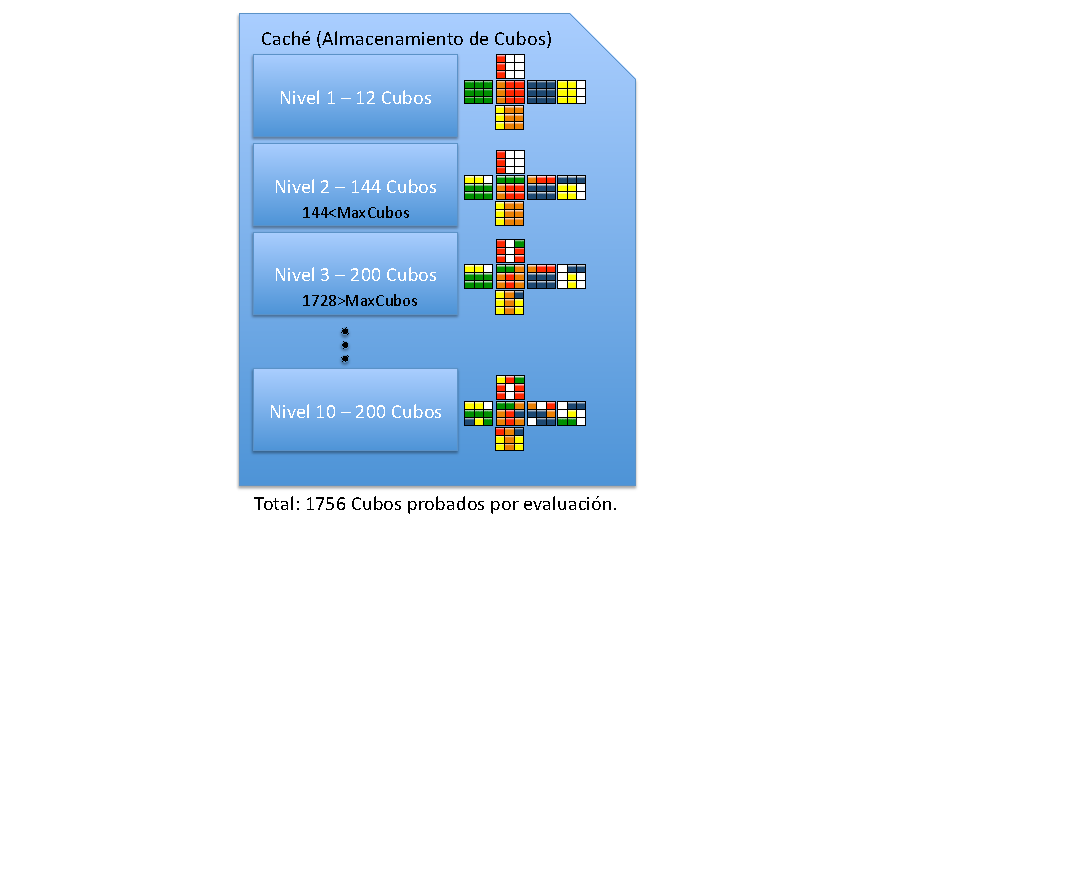
\includegraphics[width=0.45\textwidth]{figs/pdf/cache}
\caption{Almacen de cubos.}
\label{fig:cache}
\end{figure}


Además necesitamos saber la forma en la que probaremos los programas del conjunto
de entrenamiento. Como la estructura de los programas serán en forma de árbol, es
posible que en una sola iteración de la ejecución del árbol del programa no
dejemos expresar toda su capacidad resolutiva. Las sentencias que se encuentran
al principio del árbol del programa pueden no llegarse a ejecutar nunca ya que el
estado del cubo va cambiando a lo largo de la ejecución del árbol. Es por esto
que introducimos el concepto de iteraciones sobre el árbol del programa.

Para introducir las iteraciones en la ejecución del programa necesitaremos
especificar un número de iteraciones máximas para que el programa no itere
infinitamente. Además no nos interesa seguir iterando cuando hemos resuelto el
cubo. Con estas dos condiciones principales, el árbol del programa se ejecutará
una y otra vez hasta que alcancemos una solución o lleguemos a un límite de
iteraciones.

El límite de iteraciones se elegirá en función de los movimientos necesarios que
se requieren para resolver un cubo. Según estudios recientes, se cree que es
posible resolver cualquier cubo de Rubik en menos de 22 pasos. Suponiendo que al
menos se ejecuta un paso por iteración consideramos que 40 iteraciones es un
valor muy aceptable. Sin embargo, un número muy alto de iteraciones tiene un alto
coste computacional, por ello debemos elegir cautelosamente el valor adecuado de
iteraciones máximas. 

La figura \ref{fig:evaluacion} representa esquemáticamente el proceso de
evaluación.

\begin{figure}[t]
\centering
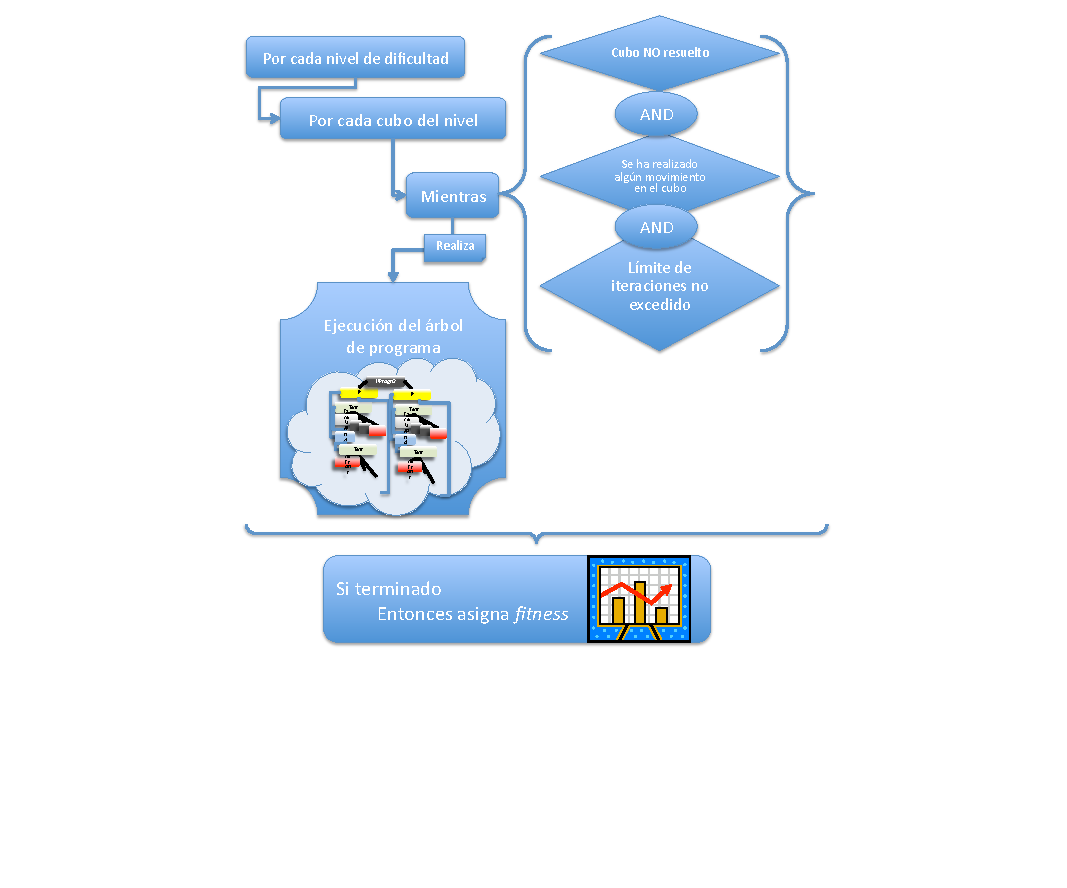
\includegraphics[width=0.85\textwidth]{figs/pdf/evaluacion}
\caption{Proceso de evaluación.}
\label{fig:evaluacion}
\end{figure}




\section{Optimización}\label{sec:optimizacion}

La programación evolutiva va estrechamente ligada a un gran consumo de recursos
computacionales. Sin embargo, no suele utilizar mucha memoria, por lo que
explotaremos al máximo el uso de la CPU generando caches y almacenando datos
calculados para que no tengan que volver a serlo.


\subsection{Reevaluación}\label{subsec:reevaluacion}

El primer paso gigantesco para acelerar el proceso de evaluación reside en no
reevaluar. Como los resultados perduran y siempre son los mismos en toda la
ejecución, no es necesario reevaluar. Así los individuos llevan un flag que
indica si han sido evaluados. Si no han sido evaluados, cuando se evalúen, se
ejecutará todo el proceso de evaluación. Si ya han sido evaluados, el proceso de
evaluación será omitido y se utilizarán los datos almacenados de la evaluación.

\subsection{Almacén de cubos}\label{subsec:almacen-cubos}

Para impedir emplear tiempo en generar cubos de Rubik cada vez que se evalua un
individuo. La muestra de cubos de Rubik de entrenamiento se generan al principio
del proceso de evolución. Así cuando evaluemos un programa, se extraerá un cubo
de Rubik del almacén de cubos. Además este sistema nos permite verificar la
calidad de los cubos que resuelven nuestros programas.

\subsection{Iteraciones inteligentes}\label{subsec:iteraciones-inteligentes}

Al introducir las iteraciones en la ejecución de los programas nos dimos cuenta
de que no siempre es necesario llegar al límite de iteraciones. Es posible que
aunque se ejecute el árbol, no se realice ningún cambio sobre el estado del cubo,
y, aunque en la siguiente iteración se vuelva a ejecutar el programa, el estado
del cubo va a ser el mismo. Por eso vamos a introducir un flag en el cubo que nos
indica si se ha cambiado el estado del cubo. Este flag se resetea en cada
iteración. Si en una iteración el flag indica que no se ha producido ningún
movimiento se escapará del bucle. No obstante, existen situaciones repetitivas,
periódicas, que son más difíciles de detectar, como por ejemplo, cuando en una
iteración se hace una acción y en la siguiente se deshace y esto se repite
infinitamente. Estos movimientos en bucle no llegan a ninguna parte. En nuestro
sistema ignoraremos estas situaciones ya que detectarlas consumiría una gran
cantidad de recursos que, si ajustamos correctamente el número de iteraciones
máximas, podemos paliar el efecto de esta situación no deseada.

\subsection{Motor del cubo de Rubik}\label{subsec:motor-cubo-rubik}

Para detectar las partes que ocupaban más tiempo del programa evolutivo, se
introdujeron temporizadores. Descubrimos que la capa de abstracción de posiciones
del cubo ocupaba gran parte del tiempo. Observamos, también, que existían
determinadas funciones equivalentes de rotación del cubo de Rubik que eran muchos
mas eficientes que otras, por lo que se reemplazaron las funciones existentes por
dichas funciones más óptimas para sacar el máximo rendimiento de ejecución.

Por otra parte, el cálculo de la entropía resultaba extrañamente pesado. La
explicación reside en que para calcular la entropía se genera un array que
contiene la situación de las pegatinas del cubo. Este array se calculaba cada vez
que se llamaba a la función de obtener las pegatinas. Ideamos un mecanismo que
mientras el cubo no cambie, el estado de las pegatinas se almacene en memoria, de
tal forma que sólo se computara el estado de las pegatinas cuando el cubo cambie
de estado.
